\ifprof
\else
La société Agronutrition est une PME du tissu économique midi-pyrénéen. Elle conçoit, 
fabrique et commercialise une large gamme de compléments nutritionnels destinés à 
améliorer la qualité et/ou le rendement des productions végétales (grandes cultures, vigne, 
arboriculture, maraîchage). Utilisables en Agriculture Biologique, ces compléments 
permettent d'améliorer les qualités nutritives des produits agricoles (teneur en protéines, 
teneur en sucres, teneur en oligo-éléments, résistance aux meurtrissures, conservation, etc.). 

L’outil industriel répond aux exigences spécifiées en terme d’Installation Classée pour la 
Protection de l’Environnement. Il est spécifiquement dédié à la formulation, la fabrication et 
le conditionnement des produits. 

L’étude se limitera à l’atelier de conditionnement des produits, aujourd’hui en partie 
automatisé.
\fi

\section{Atelier de conditionnement des produits}

\subsection{Présentation }
\ifprof
\else

Les produits réalisés par l’entreprise Agronutrition se présentent sous forme liquide et sont 
élaborés et stockés dans des cuves avant d’être conditionnés dans des bidons de 5, 10, 20 ou 
40 litres. 

\vspace{.4cm}
\begin{minipage}[c]{.53\linewidth}
Les bidons vides sont livrés par palettes. Le conditionnement des produits consiste en un 
certain nombre d’opérations réalisées sur des postes spécifiques : 
\begin{itemize}
\item poste 1 : dépalettisation des bidons vides;
\item poste 2 : remplissage des bidons;
\item poste 3 : bouchage des bidons;
\item poste 4 : marquage jet d’encre des bidons pour assurer leur traçabilité;
\item poste 5 : collage étiquette;
\item poste 6 : palettisation des bidons;
\item poste 7 : stockage des palettes pleines. 
\end{itemize}

\end{minipage} \hfill
\begin{minipage}[c]{.45\linewidth}
\begin{center}
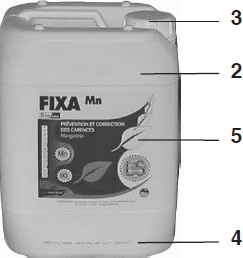
\includegraphics[width=.5\linewidth]{fig_00}
\end{center}
\end{minipage}

\vspace{.4cm}

Seules les opérations 2, 3, 4, 5 et 6 sont aujourd’hui entièrement automatisées. En particulier, 
la palettisation des bidons pleins au poste 6 est réalisée par un robot Kuka KR 180-2 PA dont 
les caractéristiques sont précisées en annexe 1.
\fi
\subsection{Schéma d’implantation}

\ifprof
\else
La Figure \label{kuka:kuka:fig:01} représente le schéma d’implantation de l’atelier de conditionnement. Les 
bidons sont déposés au poste 1 sur un tapis de transfert motorisé en mouvement continu. La 
coordination des postes est basée sur le nombre de bidons présents dans les stocks 
intermédiaires : un poste n’effectuera un cycle de production normal que si au moins un bidon 
est présent dans le stock amont et que le stock aval n’est pas saturé.

Le poste de palettisation 6 est protégé par une enceinte grillagée. Son accès est interdit durant 
les évolutions du robot par mesure de sécurité. 


\begin{figure}[H]
\centering
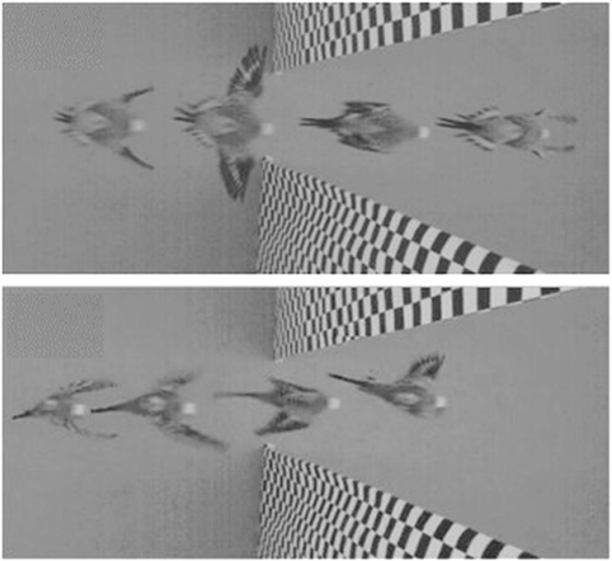
\includegraphics[width=.5\linewidth]{fig_01}
\caption{Schéma d'implantation \label{kuka:fig:01}}
\end{figure}
\fi

\subsection{Exigences du cahier des charges}
\ifprof
\else

\begin{itemize}
\item La production est de 20 000 litres de produit par jour. 
\item L’entreprise travaille 8 heures par jour. 
\item Les palettes sont aux normes européennes de dimensions (mm) : 1200x800. 
\item Le temps nécessaire au remplacement d’une palette pleine par une palette vide au 
poste 6 est estimé à 2 minutes. 
\end{itemize}
On note d’autre part (voir Figure \ref{kuka:fig:02}, page 3) :
\begin{itemize}
\item \textbf{m} : nombre de bidons rangés par longueur de palettes ; 
\item \textbf{n} : nombre de bidons rangés par largeur de palettes ; 
\item \textbf{c} : nombre de couches de bidons par palette. 
\end{itemize}
Le Tableau \ref{kuka:tab:01} indique les nombres n, m, c de bidons par palette ainsi que leurs 
dimensions $d_i$ en fonction de leur capacité. La dimension $d_3$ correspond à la hauteur d’un 
bidon. 



\vspace{.4cm}
\begin{minipage}[c]{.42\linewidth}
\begin{center}
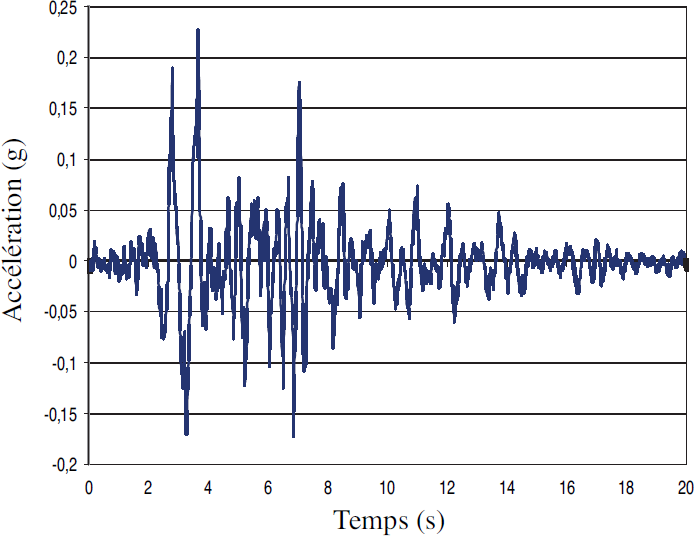
\includegraphics[width=.9\linewidth]{fig_02}
\captionof{figure}{Palette vue de dessus \label{kuka:fig:02}}
\end{center}
\end{minipage} \hfill
\begin{minipage}[c]{.55\linewidth}
\begin{center}
\begin{tabular}{lccc}
\hline
Capacité & \multicolumn{3}{c}{Conditionnement sur la palette} \\
(litres) 	& m×$d_1$ (mm)	& n×$d_2$ (mm)	& c×$d_3$ (mm)  \\
\hline
5	& 10×120	& 5×160	& 5×310 \\
10	& 6×200	& 5×160	& 4×360 \\
20	& 5×240	& 4×200	& 3×450 \\
40	& 4×300	& 4×200	& 2×720 \\
\hline
\end{tabular}
\captionof{table}{Caractéristiques des bidons suivant leur capacité \label{kuka:tab:01}}
\end{center} 

\end{minipage}

\vspace{.4cm}


On se place dans le cas le plus défavorable, c'est-à-dire celui consistant à 
palettiser des bidons de 5 litres. On se propose de déterminer la durée maximale nécessaire à 
la dépose d’un bidon sur la palette. 
\fi

\question{À partir des données définies dans le cahier des charges, déterminer le nombre de bidons de 5 litres à palettiser par jour.}
\ifprof
\begin{corrige}
Le cahier des charges impose une production de 20000\si{L/j}, à raison de bidons de \SI{5}{L}, cela 
représente donc : 20000/5=4000 bidons/jours.
\end{corrige}
\else
\fi

\question{À partir des données définies dans le cahier des charges, en déduire le nombre de palettes à produire par jour.}
\ifprof
\begin{corrige}
Le tableau 1 donne alors : $m\times n \times c=10x5x5=\SI{250}{Bidons/palettes}$. 
Il faut donc produire :4000/250=16 palettes/jours.
\end{corrige}
\else
\fi

\question{À partir des données définies dans le cahier des charges, en déduire le temps nécessaire à la composition d’une palette en minutes incluant le temps de changement d’une palette.}
\ifprof
\begin{corrige}
Sur une production de \SI{8}{h}, on a donc seulement \SI{30}{min} à consacrer par palette. 
Le temps de transfert étant de \SI{2}{min}, il ne reste donc que \SI{28}{min} pour la remplir.
\end{corrige}
\else
\fi

\question{À partir des données définies dans le cahier des charges, en déduire la durée maximale nécessaire à la dépose d’un bidon sur la palette en  secondes.}
\ifprof
\begin{corrige}
Pour 250 bidons, cela représente alors \SI{1680}{s}/250=\SI{6,72}{s/bidon}.
\end{corrige}
\else
\fi


\section{Etude de la palettisation 6}

\ifprof
\else

\vspace{.4cm}
\noindent\begin{minipage}[c]{.53\linewidth}
La pièce maîtresse du poste 6 est un robot de palettisation Kuka KR 180-2 PA (voir annexe 1). Ses fonctions de service (voir Figure \ref{kuka:fig:03}) sont définies ci-après : 
\begin{itemize}
\item FP1 : Déposer les bidons sur la palette;
\item FP2 : Déposer les cartons sur la palette (fonction non étudiée);
\item FS3 : Piloter le robot;
\item FS4 : Alimenter en énergie électrique les actionneurs;
\item FS5 : Protéger l’environnement lors des évolutions du robot.
\end{itemize}

\end{minipage} \hfill
\begin{minipage}[c]{.45\linewidth}
\begin{center}
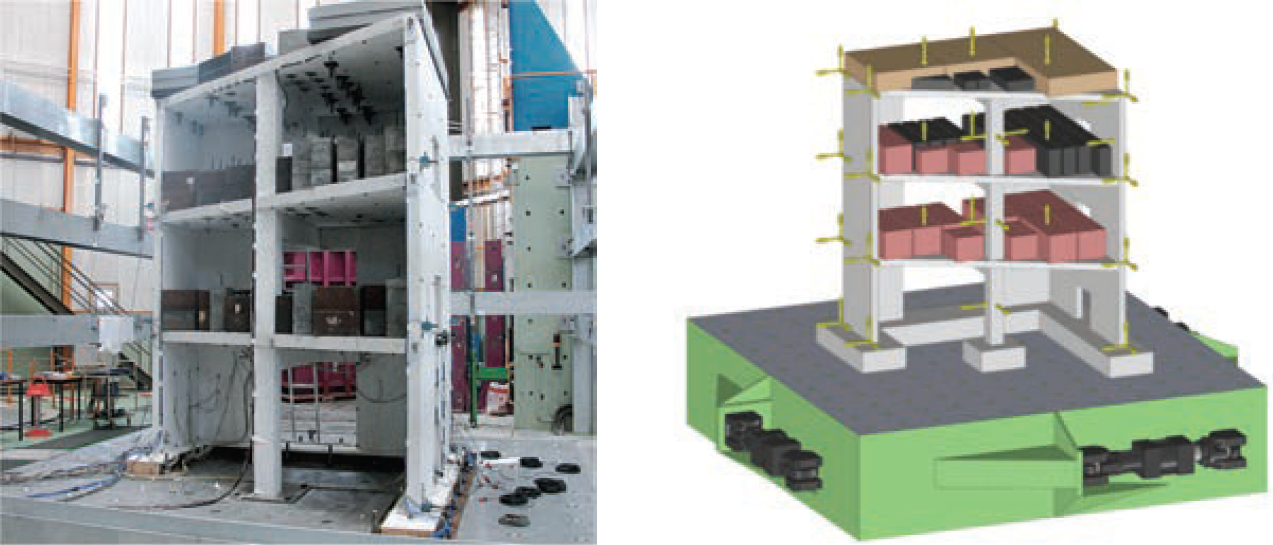
\includegraphics[width=.9\linewidth]{fig_03}
\captionof{figure}{Diagramme des interacteurs \label{kuka:fig:03}}
\end{center}
\end{minipage}

\vspace{.4cm}
\fi


\subsection{Objectif }

\ifprof
\else
On se propose de vérifier que les caractéristiques du robot permettent de satisfaire la cadence 
de production imposée par le cahier des charges. 
\fi

\subsection{Données \label{sec:2-2}}

\ifprof
\else

\begin{itemize}
\item Le temps $t_{P2}$ de remplissage d’un bidon de 5 litres au poste 2 est de 6 secondes. 
\item Le temps $t_{P3}$ de bouchage d’un bidon au poste 3 est de 3 secondes. 
\item Les opérations associées aux postes 4 et 5 se font à la << volée >>, sans arrêt du bidon,
leur durée est donc négligeable. 
%\item Le grafcet de la Figure 16, annexe 2, représente le fonctionnement normal du  poste de palettisation. 
\item Les positions du robot sont spécifiées dans l’annexe 3, 
ainsi que les étapes correspondantes du grafcet de fonctionnement normal. 
\item Dans la position de référence notée $P_0$, $\alpha_1 = -45\degres$ (voir Figure 13, annexe 1, la signification de l’angle $\alpha_1$). 
\end{itemize}
\fi

\subsection{Détermination de la cadence de production}
\ifprof
\else

Une simulation a permis d’estimer les amplitudes des déplacements des différents axes $A_i$ du robot lors de la dépose d’un bidon sur la palette. 

Afin de déterminer la durée d’un déplacement, seul est pris en compte, parmi les axes $A_i$ sollicités, celui dont l’amplitude, en valeur absolue, est la plus importante lors de ce déplacement. Les résultats sont consignés dans le Tableau \label{kuka:tab:02}. 

Le profil de vitesse imposé lors de ces déplacements est représenté Figure \ref{kuka:fig:04}.

\begin{figure}[!h]
\centering
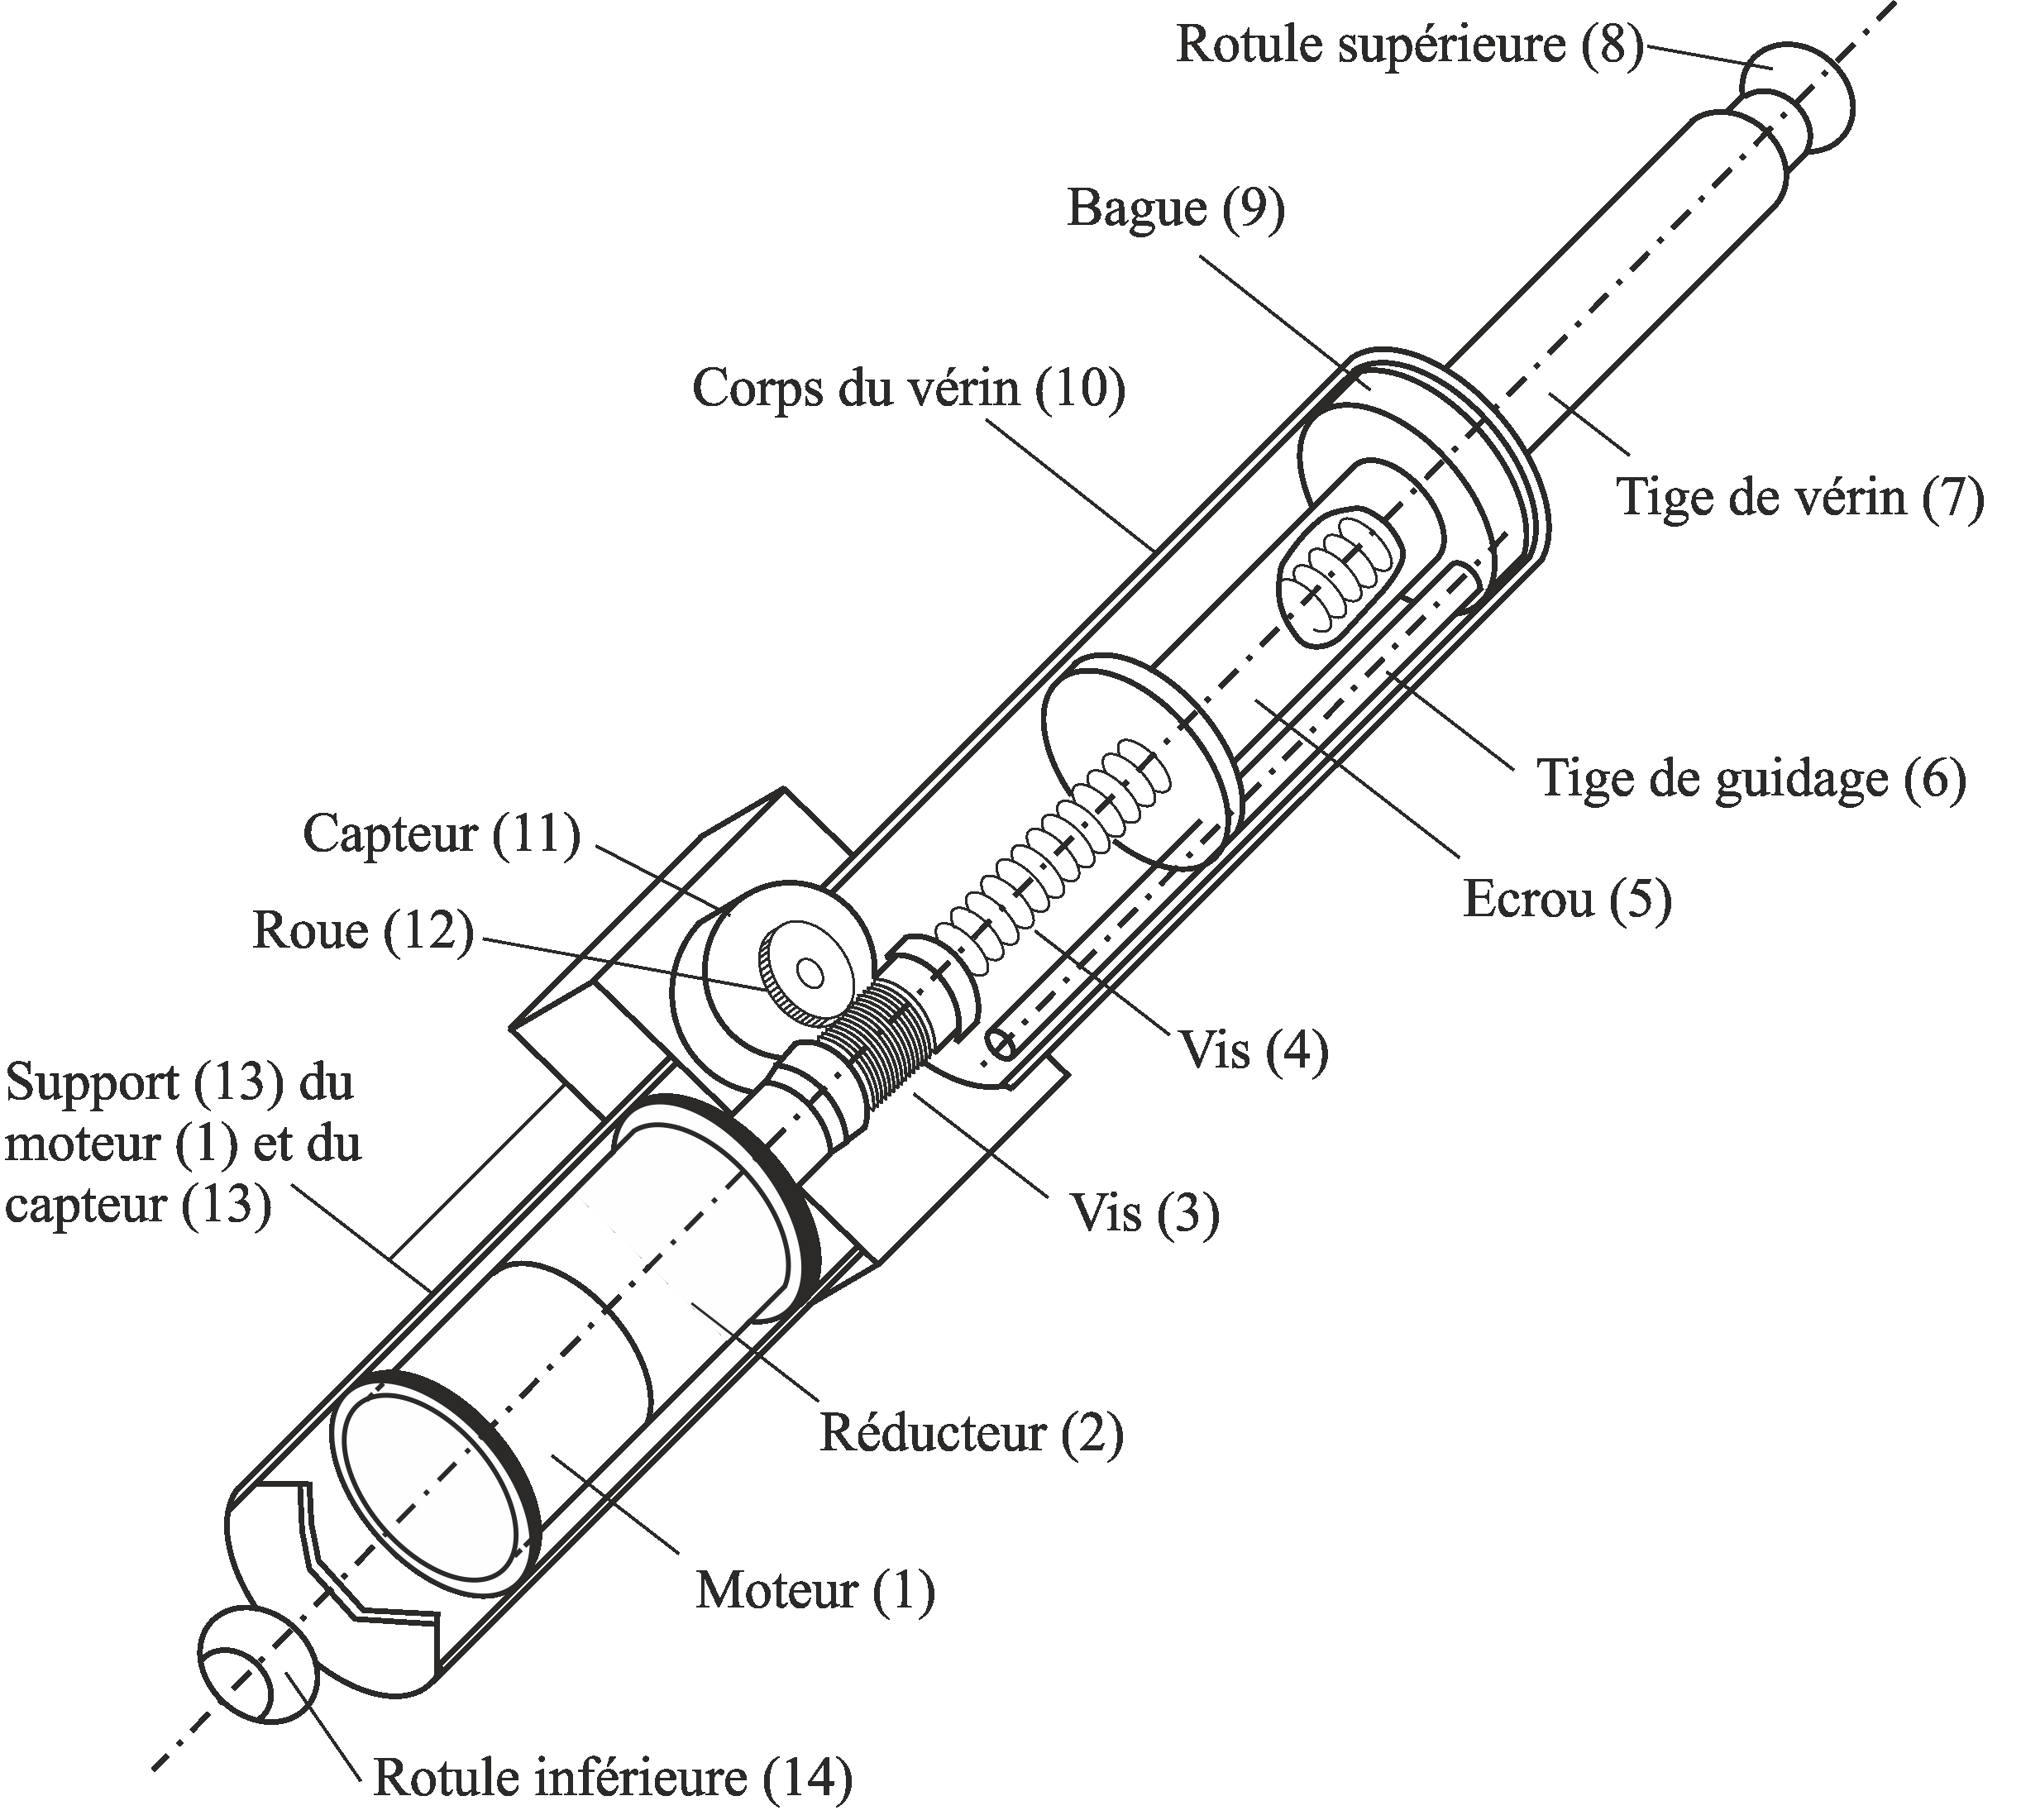
\includegraphics[width=.5\linewidth]{fig_04}
\caption{Profil des vitesses  \label{kuka:fig:04}}
\end{figure}
\fi

\question{\label{q2-1}Déterminer, pour les cas 2 et 3 définis dans le Tableau \ref{kuka:tab:02}, la durée 
$d_i$ des différentes phases du profil de vitesse. En déduire le temps total $T_t$ nécessaire à ces 
déplacements. Les résultats seront reportés dans le tableau suivant qui sera recopié sur votre copie.}
\ifprof
\begin{corrige}
Le temps pour atteindre $\indice{\omega}{max}$ est de $\SI{0,35}{s}$.
Dans le profil de vitesse, l'angle parcouru correpond à l'aire sous la courbe. 
L'angle nécessaire pour atteindre pour atteindre $\indice{\omega}{max}$ puis décélérer est donc de :
$t_1 \indice{\omega}{max} = 0,35 \times 105 = 36,75 \degres$.

Dans le cas 2, on a donc :
\begin{itemize}
\item $t_1 = \SI{0,35}{s}$, 
\item $d_2 =  \dfrac{90-36,75}{105} =  \SI{0,5}{s}$;
\item $d_3 = t_1 =  \SI{0,35}{s}$.
\end{itemize}

Dans le cas 3, l'angle à parcourir est inférieur à $36,75 \degres$.
La vitesse maximale n'est donc pas atteinte. 

Dans ces conditions, le profil de vitesse est un triangle. L'aire sous le triangle correspond à l'angle à parcouri. 
On a donc $\alpha = t_1 v_1$ et $v_1/t_1 = \indice{\omegap}{max}$.
On a alors $\alpha = t_1^2 \indice{\omegap}{max}$ soit $t_1 =\sqrt{\dfrac{\alpha}{\indice{\omegap}{max}}} = \sqrt{15/300} = \SI{0,22}{s}$. Par suite : 
\begin{itemize}
\item $t_1 = \SI{0,22}{s}$, 
\item $d_2 =  \SI{0}{s}$;
\item $d_3 =  \SI{0,22}{s}$;
\item $T_t = \SI{0,44}{s}$.
\end{itemize}

\end{corrige}
\else
\fi

\ifprof
\else

\begin{center}
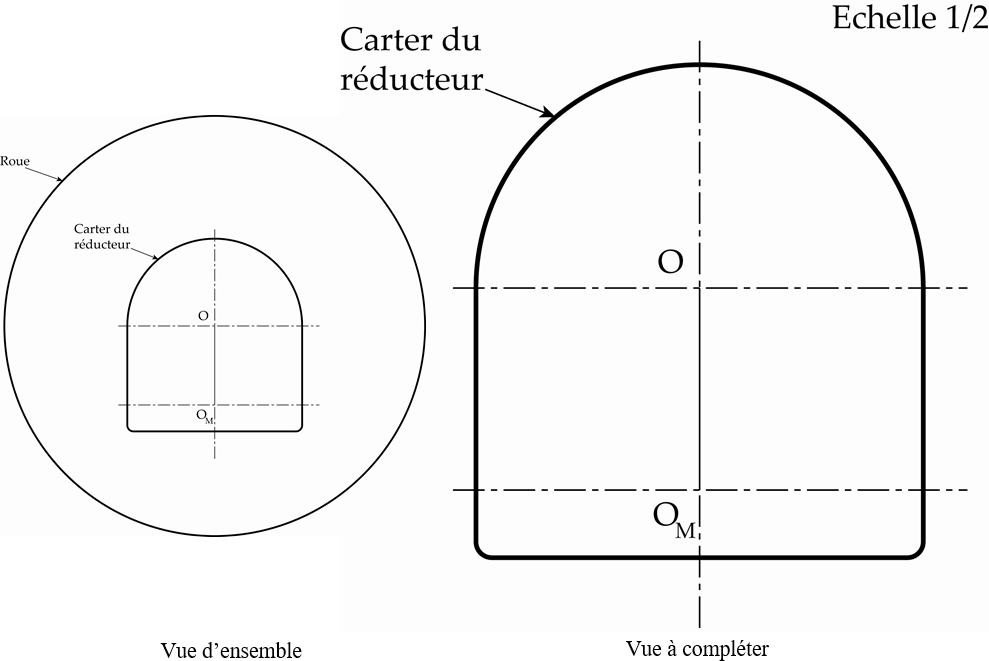
\includegraphics[width=.7\linewidth]{dr_02}
\end{center}


\begin{table}[!h]
\centering
\begin{tabular}{llcccc}
\hline
Cas & Déplacements & Axe & Amplitude  & $\omega_{\text{max}}$ &  $\dot{\omega}_{\text{max}} $\\
&&&maximale & $ \si{\degres/s}$ & $ \si{\degres/s^2}$ \\
\hline
1 & $P_0$ à $P_1$, $P_1$ à $P_0$ & $A_1$ & 45\degres & 105 & 300 \\  
2 & $P_1$ à $P_i$                                  & $A_1$ & 90\degres & 105 & 300 \\ 
3 & $P_1$ à $P_2$, $P_2$ à $P_1$,
      $P_i$ à $P_j$, $P_j$ à $P_i$,   & $A_3$ & 15\degres & 105 & 300 \\
\hline
\end{tabular}
\caption{Amplitudes maximales lors des déplacements \label{kuka:tab:02}}
\end{table} 



Nota : Indépendamment des valeurs calculées question \ref{q2-1}, on retiendra, pour la suite 
du sujet, les durées suivantes des différentes opérations :

\begin{center}
\begin{tabular}{lll}
\hline
Étapes	& Opérations 			& Durée Tt (s) 	\\
\hline
1	& Déplacer le robot de P0 à P1 	& 0,8 		\\
3 et 5 	& Déplacer le robot de P1 à P2 ou de P2 à P1 & 0,5 \\ 
4 	& Prendre un bidon 		& 0,1 \\ 
9 	& Déplacer le robot de P1 à Pi 	& 1,2 \\
10 et 12 & Déplacer le robot de Pi à Pj ou de Pj à Pi & 0,5 \\ 
11 	& Déposer un bidon 		& 0,1 \\ 
13 	& Déplacer le robot de Pi à P0 	& 0,8 \\
\hline
\end{tabular}
\end{center}

Le temps nécessaire à la détermination de la position Pi lors de l’étape 8 est négligeable. 
\fi

\question{ En supposant nul le temps d’attente d’un bidon lors de l’étape 2, déterminer 
le temps $t_{P6}$ nécessaire à la dépose d’un bidon sur la palette, temps nécessaire au robot pour 
partir de la position P0 et revenir en P0. }
\ifprof
\begin{corrige}
L'ordre des mouvements est le suivant : $P_0 \rightarrow P_1 \rightarrow P_2 \rightarrow \text{Prise} \rightarrow P_1\rightarrow P_i \rightarrow P_k \rightarrow \text{Dépose} \rightarrow P_i \rightarrow P_0 $.
 Soit $0,8 + 0,5 + 0,1 + 0,5 + 1,2 + 0,5 + 0,1 + 0,5 + 0,8$ soit un total de \SI{5}{s}.
\end{corrige}
\else
\fi

\ifprof
\else

On considère comme instant initial l’instant où le premier bidon arrive au poste 6 suite à la 
mise en route du système de conditionnement. Le niveau $Q(t)$ du stock de bidons en amont du 
poste 6 évolue alors comme indiqué Figure \ref{kuka:fig:05} avec :
\begin{itemize}
\item phase 1 : Chargement palette 1 
\item phase 2 : Evacuation palette 1 
\item phases 3 4 : Chargement palette 2 
\item phase 5 : Evacuation palette 2.
\end{itemize}

Le cycle se reproduit ensuite identique à lui-même pour les autres palettes. 


\begin{figure}[H]
\centering
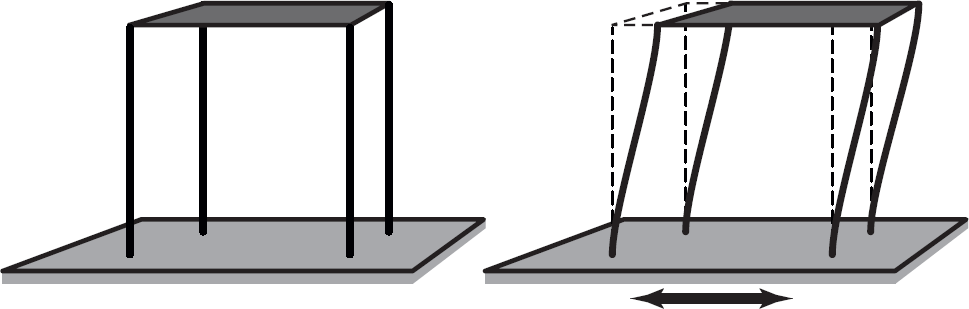
\includegraphics[width=.75\linewidth]{fig_05}
\caption{Evolution du stock en amont du poste 6\label{kuka:fig:05}}
\end{figure}
\fi


\question{En considérant la durée des opérations $t_{P2}$ et $t_{P3}$ définies paragraphe \ref{sec:2-2}, 
justifier que le niveau du stock n’évolue pas lors de la phase 1. Quel est alors le temps 
d’attente d’un bidon lors de l’étape 2 ?}
\ifprof
\begin{corrige}
Les opération s’effectuant en série et à flux tendu, c’est le temps le plus important qui 
conditionne la ligne, or $tp_2=\SI{6}{s}$, $tp_3=\SI{3}{s}$, $tp_6=\SI{5}{s}$. 

Un bidon arrive donc toutes les \SI{6}{s} au robot ce qui lui laisse le temps de le palettiser et de 
revenir en place en $P_0$. 

Il n’y a donc pas de stock sur la ligne et le temps d’attente à l’étape 2 est donc nul. 
\end{corrige}
\else
\fi

\question{Déterminer le niveau $\indice{Q}{max}$ du stock amont atteint lors de la phase 2. La 
longueur de 4 mètres de la zone de stockage amont du poste 6 est-elle suffisante ?}
\ifprof
\begin{corrige}
Pendant le changement de palette, les bidons ne sont plus chargés et s’accumulent donc à 
raison de 1 toutes les \SI{6}{s}. 
En \SI{2}{mn}, on a donc $120/6=20$ bidons de stockés, soit $\indice{Q}{max}=20$.

D’après la figure 1, nous savons que les bidons sont disposés suivant leur longueur. 
Nous avons donc une longueurs stockée de $20\times d_1=\SI{2400}{mm}<\SI{4000}{mm}$. 
La capacité de stockage est donc suffisante.
\end{corrige}
\else
\fi

\question{Déterminer :}
\vspace{-.4cm}
\textit{
\begin{enumerate}
\item la durée $t_3$ de la phase 3 ; 
\item le nombre de bidons chargés sur la palette lors de cette phase ; 
\item la durée $t_4$ de la phase 4.
\end{enumerate}}
\ifprof
\begin{corrige}
On ne récupère que $6-5=\SI{1}{s}$ par transfert, il faut donc 120 bidons transférés pour regagner les 
\SI{120}{s} de perdues, soit $120 \times \SI{5}{s}=\SI{600}{s}$, soit $t_3=\SI{10}{mn}$.
Ayant alors chargé 120 bidons, il en reste alors 250-120=130 à charger. 
On a donc $t_4=130x5=\SI{10}{mn}\SI{50}{s}$. 
\end{corrige}
\else
\fi

\question{En déduire le temps nécessaire à la formation d’une palette correspondant 
à la durée des phases 3, 4 et 5. Conclure quant à la satisfaction du cahier des charges.}
\ifprof
\begin{corrige}
Le temps de cycle est donné par $t_3+t_4+t_5=\SI{22}{mn}\SI{50}{s}<\SI{30}{mn}$, la fonction est donc validée.
\end{corrige}
\else
\fi

%3 
\section{Vérification du système de freinage du robot}
%3.1 
\subsection{Objectif }
\ifprof
\else

Suite à l’ouverture inopinée du portail d’accès au poste 6 ou à l’appui sur le bouton d’arrêt 
d’urgence, le robot doit immédiatement s’immobiliser dans la position courante. On souhaite 
alors vérifier que les freins équipant le robot sont suffisants pour assurer sa configuration 
d’équilibre dans le cas d’une charge maximale de \SI{50}{daN} (préhenseur + bidon de 40 litres) et 
qu’il ne faudra pas mettre des actionneurs en parallèle.
\fi


%3.2 
\subsection{Données}
\ifprof
\else
On se place dans la situation particulière définie Figure \ref{kuka:fig:06} avec $\alpha_2= -\SI{90}{\degres}$ et $\alpha_3= +\SI{90}{\degres}$.

\begin{figure}[!h]
\centering
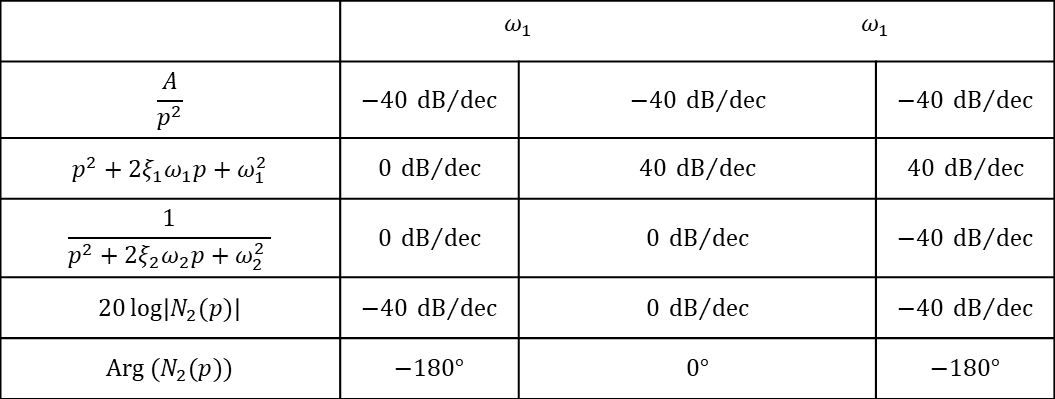
\includegraphics[width=.5\linewidth]{fig_06}
\caption{Configuration particulière du robot\label{kuka:fig:06}}
\end{figure}


On donne : 
\begin{itemize}
\item $O_2O_3 = O_6O_7 = \SI{1250}{mm}$; 
\item $O_3O_{10} = O_8O_9 = \SI{1350}{mm}$; 
\item $O_2O_6 = O_3O_7 = O_3O_8 = O_9O_{10} = \SI{500}{mm}$; 
\item $\vect{P} = -500\vect{z_4}$. 
\end{itemize}

On admettra pour simplifier que le point $O_4$ est situé sur l’axe $\vect{x_3}$ et que l’axe $\vect{z_4}$ passe par le point $O_9$. De même, les poids propres des pièces seront négligés par rapport aux autres 
actions. 

Les liaisons pivot sont supposées parfaites (pas de frottement). 

Les couples de freinage maxi $M_{f2}$ et $M_{f3}$ des freins associés aux moteurs $M_2$ et $M_3$ sont de 
\SI{5}{mN} sur l’arbre moteur. On leur adjoint en série un réducteur de rapport 1/200.
\fi

\question{Déterminer les actions de la barre 8 et du bras 3 sur le poignet 4. }
\ifprof
\begin{corrige}
Le problème est plan. 
\begin{itemize}
\item On isole la barre 8.
\item BAME : 
\begin{itemize}
\item Pivot $\torseurstat{T}{4}{8} = \torseurl{\vectf{4}{8}}{\vect{0}}{O_9}$ glisseur.
\item Pivot $\torseurstat{T}{7}{8} = \torseurl{\vectf{7}{8}}{\vect{0}}{O_8}$ glisseur.
\end{itemize}
\item D'après le PFS, 8 étant soumis à deux glisseurs, on a donc $\vectf{4}{8}=-\vectf{7}{8}=F_{48} \vect{x_3}$.
\end{itemize}

\vspace{.5cm}

\begin{itemize}
\item On isole le bras 4.
\item BAME : 
\begin{itemize}
\item Pivot $\torseurstat{T}{8}{4} = \torseurl{-F_{48}\vect{x_3} }{\vect{0}}{O_9}$.
\item Pivot $\torseurstat{T}{3}{4} = \torseurl{\vectf{3}{4}}{\vect{0}}{O_8}$.
\item Pesanteur $\torseurstat{T}{\text{Pes}}{4} = \torseurl{\vect{P}}{\vect{0}}{O_4}$.
\end{itemize}
\item On applique le PFS en $O_{10}$ :
\begin{itemize}
\item TRS sur $\vect{x_4}$ : $-F_{48}+X_{34} = 0$;
\item TRS sur $\vect{z_4}$ : $-500+Y_{34} = 0$;
\item TMS en $O_{10}$ sur $\vect{y_4}$ : $P\times 500 \cos 40 -500F_{48} \sin 40 = 0$.
\end{itemize}  
\item Résolution : $F_{48} =  X_{34} = \dfrac{P}{\tan 40} $.
\end{itemize}
\end{corrige}
\else
\fi

\question{En isolant l’ensemble 3 et 4 et en considérant les informations fournies Tableau 4, annexe 1, déterminer l’expression du moment $M_{f3}$ correspondant à l’action du frein sur la pièce 3 en $O_3$.}
\ifprof
\begin{corrige}
\begin{itemize}
\item On isole l'ensemble (3+4).
\item BAME : 
\begin{itemize}
\item pivot en $O_{3}$ $\torseurstat{T}{2}{3}$;
\item pivot en $O_{9}$ $\torseurstat{T}{8}{4}$;
\item frein en $O_{3}$;
\item pesanteur en $O_{4}$ $\torseurstat{T}{\text{pes}}{4}$;
\end{itemize}
\item pour caractériser le moment de freinage sans faire intervenir $\torseurstat{T}{2}{3}$, on réalise un théorème du moment statique en $O_3$ en projection sur $\vect{y}$: 
$$
M_{f3} + P(1350+500\cos 40) -F_{48}500\sin 40 = 0. 
$$
Oa donc 
$M_{f3} =- P(1350+500\cos 40) +P\dfrac{\cos 40}{ \sin 40}500\sin 40  
= - 1350P- P 500\cos 40 +P 500 \cos 40
= - 1350P$.

$M_{f3} = \SI{675}{Nm}$

\end{itemize}
\end{corrige}
\else
\fi

Le dispositif de freinage ne permet qu’un couple maxi de \SI{5}{Nm} sur l’axe 
moteur. 


\question{Quel est alors le couple de freinage disponible en sortie du réducteur ? }
\ifprof
\begin{corrige}
Avec un réducteur de 200, le couple de freinage est de $200\times 5 = \SI{1000}{Nm}$.
\end{corrige}
\else
\fi

\question{Le maintien du freinage est-il assuré ?}
\ifprof
\begin{corrige}
Le moteur permet bien de freiner la charge $\SI{1000}{Nm} > \SI{675}{Nm}$.

\end{corrige}
\else
\fi

On veut alors vérifier que le dispositif de freinage du moteur $M_2$ convient. 

\question{En isolant la pièce 7, déterminer l’action de la barre 6 sur la pièce 7. }
\ifprof
\begin{corrige}
\begin{itemize}
\item On isole la pièce 7.
\item BAME : 
\begin{itemize}
\item pivot en $O_{8}$ $\torseurstat{T}{8}{7}$ tel que $\vectf{8}{7}= F_{87} \vect{x_4}$ (8 soumis à 2 glisseurs -- de plus $F_{48}+F_{78}=0\Rightarrow F_{87}=F_{48}= \dfrac{P}{\tan 40}$);
\item pivot en $O_{7}$ $\torseurstat{T}{6}{7}$ tel que $\vectf{6}{7}= F_{67} \vect{z_4}$ (6 soumis à 2 glisseurs);
\item pivot en $O_{3}$ 	;
\end{itemize}
\item  on réalise un théorème du moment statique en $O_3$ en projection sur $\vect{y}$: 
$$
-F_{87}500\sin 40 -F_{67}500\cos 30  = 0. 
$$
Oa donc 
$F_{67}  = -\dfrac{P}{\tan 40}\dfrac{\sin 40}{\cos 30}  = -\dfrac{P}{\cos 40}{\cos 30} $.

\end{itemize}
\end{corrige}
\else
\fi

\question{En considérant l’ensemble 2, 3, 4, 7, 8, déterminer l’expression du moment $M_{f2}$
correspondant à l’action du frein sur la pièce 2 en $O_2$. Calculer $M_{f2}$.}
\ifprof
\begin{corrige}
\begin{itemize}
\item On isole 2, 3, 4, 7, 8.
\item BAME : 
\begin{itemize}
\item pesanteur en $O_4$
\item pivot en $O_{7}$ $\torseurstat{T}{6}{7}$;
\item pivot en $O_{2}$ $\torseurstat{T}{1}{2}$.
\end{itemize}
\item  on réalise un théorème du moment statique en $O_2$ en projection sur $\vect{y}$ et on obtient 
$M_{f2}=-1350P = -\SI{675}{Nm}$.
\end{itemize}

\end{corrige}
\else
\fi

\question{Le dispositif de freinage étant identique à celui de l’axe 3, le maintien du freinage 
est-il assuré ?}
\ifprof
\begin{corrige}
Le maintien du freinage est assuré.
\end{corrige}
\else
\fi

\section{Analyse cinématique du robot}

\subsection{Objectif}
\ifprof\else
On souhaite tout d’abord s’assurer que, pour tous les conditionnements de produit, le robot 
pourra mettre en position le bidon le plus éloigné situé dans les coins du bord extérieur de la 
palette. 

On s’intéressera ensuite aux particularités des mouvements du robot (dont la vocation est la 
palettisation) résultant de l’utilisation d’un double parallélogramme. 
\fi

\subsection{Données} 
\ifprof\else
\begin{itemize}
\item L’espace de travail du robot est défini Figure 15, annexe 1. 
\item Les palettes sont disposées symétriquement par rapport à l’axe $\axe{O_0}{x_0}$ (voir Figure \ref{kuka:fig:01}) et leur bord intérieur est situé à une distance de 1,6 mètre du point $O_0$. 
\item On suppose que l’axe vertical de symétrie d’un bidon est confondu avec l’axe $\axe{O_4}{z_4}$
et que la face supérieure d’un bidon est située dans le plan $\angl{x_4}{z_4}$. 
\item Distance d’approche $P_iP_j$ = $0,5 \times$ hauteur d’un bidon.%(voir grafcet annexe 2). 
\item Le plan supérieur de la palette est situé à une hauteur de \SI{200}{mm} du sol. 
\end{itemize}
\fi

\question{A partir des données précédentes, en déduire pour quel type de bidon le 
conditionnement est le plus critique.}
\ifprof
\begin{corrige}
Bidon de 40 L.
\end{corrige}
\else
\fi


\question{Représenter sur la figure 17*** du document réponse DR1 la palette pleine (un tracé à 
main levée est suffisant).}


\question{Indiquer sur ce document les coordonnées $x_4$, $y_4$, $z_4$ du point $O_4$ dans le cas (ou les 
cas) le plus défavorable. Conclure. }

On se place dans la position instantanée de la Figure \ref{kuka:fig:06}, en supposant les 
différents moteurs alimentés et en désignant par $\omega_{ij}$ la vitesse angulaire du solide $i$ par 
rapport au solide $j$.

\question{Déterminer $\vect{V}\left(O_4/7\right)$,  vitesse de $O_4$ par rapport à 7.}
\ifprof
\begin{corrige}
$\vect{V}\left(O_4/7\right) = \deriv{\vect{O_3O_4}}{\rep{7}} = O_3 O_4 \deriv{\vect{x_3}}{\rep{7}}$
\end{corrige}
\else
\fi

\question{Déterminer $\vectv{O_4}{7}{1}$,  vitesse de $O_4$ appartenant à 7 par rapport à 1.}
\ifprof
\begin{corrige}
$\vectv{O_4}{7}{1}$
$=\vectv{O_3}{7}{1}$
$=\vectv{O_2}{7}{1} + \vect{O_3O_2} \wedge \omega_{21} \vect{y_3}=O_2O_3\omega_{21} \vect{x_3}$
\end{corrige}
\else
\fi

\question{Déterminer $\vectv{O_4}{1}{0}$,  vitesse de $O_4$ appartenant à 1 par rapport au sol.}
\ifprof


\begin{corrige}
$\vectv{O_4}{1}{0}$
$=\vectv{O_1}{1}{0} + \vect{O_4O_1} \wedge \omega_{10} \vect{z_1}=-(1700+500\cos 40) \omega_{10} \vect{y_3}$
\end{corrige}
\else
\fi

\question{En déduire la nature du mouvement du poignet 4 par rapport à la pièce 1. }
\ifprof
\begin{corrige}
Le poignet 4 a donc, par rapport à 1, un mouvement de translation en $\vz{3}$ et en $\vx{3}$ ainsi qu’une 
rotation autour de $\axe{O_1}{z_1}$.
\end{corrige}
\else
\fi

\question{Ceci correspond-il à la vocation de palettisation du robot ? }
\ifprof
\begin{corrige}
Oui, cela convient très bien à sa fonction de palettisation. 
\end{corrige}
\else
\fi

\question{Quel est l’intérêt d’une telle structure par rapport à celle d’un robot 6 axes  (voir Figure \ref{kuka:fig:07}) ?}
\ifprof
\begin{corrige}
L’intérêt par rapport à un robot 6 axes est avant tout une question de coût car dans ce cas les 
rotations des axes A4, A5 et A6 sont inutiles.
\end{corrige}
\else
\fi


\ifprof
\else
\begin{figure}[!h]
\centering
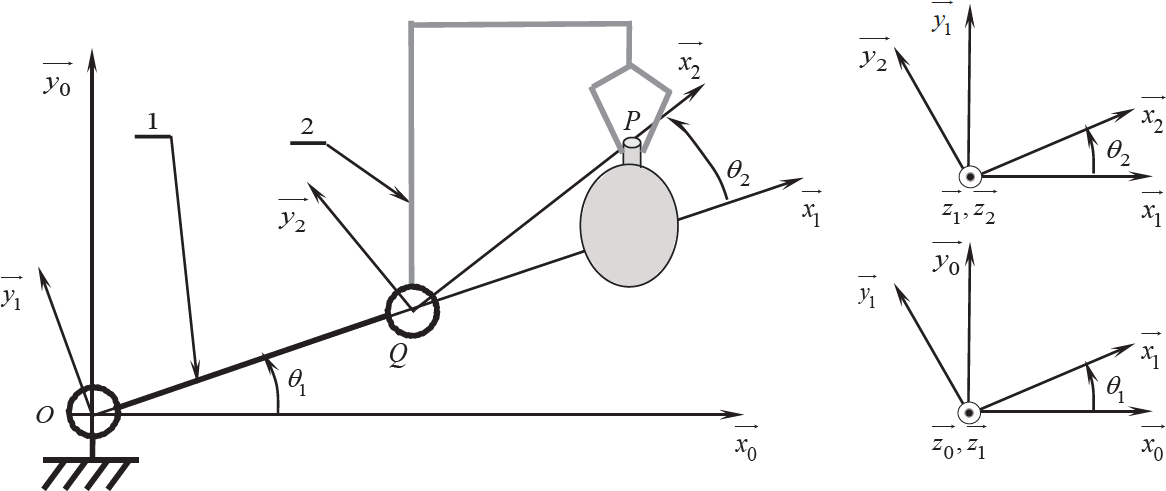
\includegraphics[width=.5\linewidth]{fig_07}
\caption{Robot 6 axes \label{kuka:fig:07}}
\end{figure}
\fi


%6 ASSERVISSEMENT EN POSITION DE L’AXE A1 
\section{Asservissement en position de l'axe A1}

\subsection{Objectif}
\ifprof
\else
On s’intéresse à l’asservissement en position de l’axe A1. On souhaite s’assurer que la chaîne 
fonctionnelle d’asservissement permet de respecter les performances souhaitées en terme de 
précision, rapidité et stabilité tout en restant peu sensible aux variations de l’inertie du robot 
suivant la charge transportée. 
\fi

\subsection{Données \label{sec:6:2}} 
\ifprof
\else
L’axe A1 est mu par un servomoteur qui présente l'avantage de posséder une très faible 
inertie. Le comportement électromécanique de ce type de moteur est donné par les équations 
suivantes : 
\begin{itemize}%[$\bullet$]
\item $u(t) = Ri(t) + e(t)$ (1);
\item $e(t) = k_e \omega_m(t)$  (2);
\item $J_e \dfrac{\d \omega_m(t)}{\d t} = c_m(t)$ (3);
\item $c_m(t) = k_t i(t)$ (4).
\end{itemize}

Avec $u(t)$ la tension appliquée aux bornes du moteur, $i(t)$ le courant d’induit, $e(t)$ la force 
contre électromotrice, $\omega_m(t)$ la vitesse de rotation du moteur, $c_m(t)$ le couple délivré par le 
moteur et $J_e$ l’inertie équivalente ramenée sur l’arbre moteur. 

Le réducteur retenu pour cette motorisation est un réducteur Harmonic-Drive. Les 
caractéristiques de l’ensemble moteur-réducteur sont les suivantes : 
\begin{itemize}
\item $k_e = \SI{0,2}{V/(rad/s)}$ : constante de force électromotrice ; 
\item $k_t = \SI{0,2}{Nm/A}$ : constante de couple ; 
\item $R = \SI{2}{\Omega}$ : résistance de l’induit ; 
\item $J_m = \SI{4e-3}{kg.m^2}$ : inertie de l’ensemble axe moteur et réducteur sur l'arbre moteur ; 
\item $N = 200$ : rapport de transmission. 
\end{itemize}

L’inertie $J_1$ du robot autour de l’axe $\axe{O_1}{z_1}$ dépend de la configuration du robot et de la masse
transportée. Elle est telle que : 
\begin{itemize}
\item $J_1 \text{mini} = \SI{50}{kg.m^2}$  lorsque le déplacement a lieu à vide ; 
\item $J_1 \text{maxi} = \SI{200}{kg.m^2}$  lorsque la masse transportée est de \SI{50}{daN}. 
\end{itemize}
L’inertie équivalente $J_e$ ramenée sur l’arbre moteur est alors égale à : 
\begin{itemize}
\item $J_e \text{mini} = \SI{5,25e-3}{kg.m^2}$  lorsque $J_1 = J_1 \text{mini}$; 
\item $J_e \text{maxi} = \SI{9e-3}{kg.m^2}$  lorsque $J_1 = J_1 \text{maxi}$. 
\end{itemize}

La chaîne fonctionnelle de l’asservissement de l’axe A1 est représentée Figure \ref{kuka:fig:08}. 

La boucle interne réalise une correction de vitesse à partir de la tension $u_g(t)$ fournie par une 
génératrice tachymétrique de gain $K_g$ montée en prise directe sur le moteur. $G$ est le gain 
réglable de l’amplificateur de puissance. 

La boucle externe réalise la correction de position à partir de la tension $u_r(t)$ fournie par le 
capteur de position de gain $K_r$ monté en prise directe sur l’arbre de sortie du réducteur. La 
fonction de transfert du correcteur est notée $C(p)$.

\begin{figure}[!h]
\centering
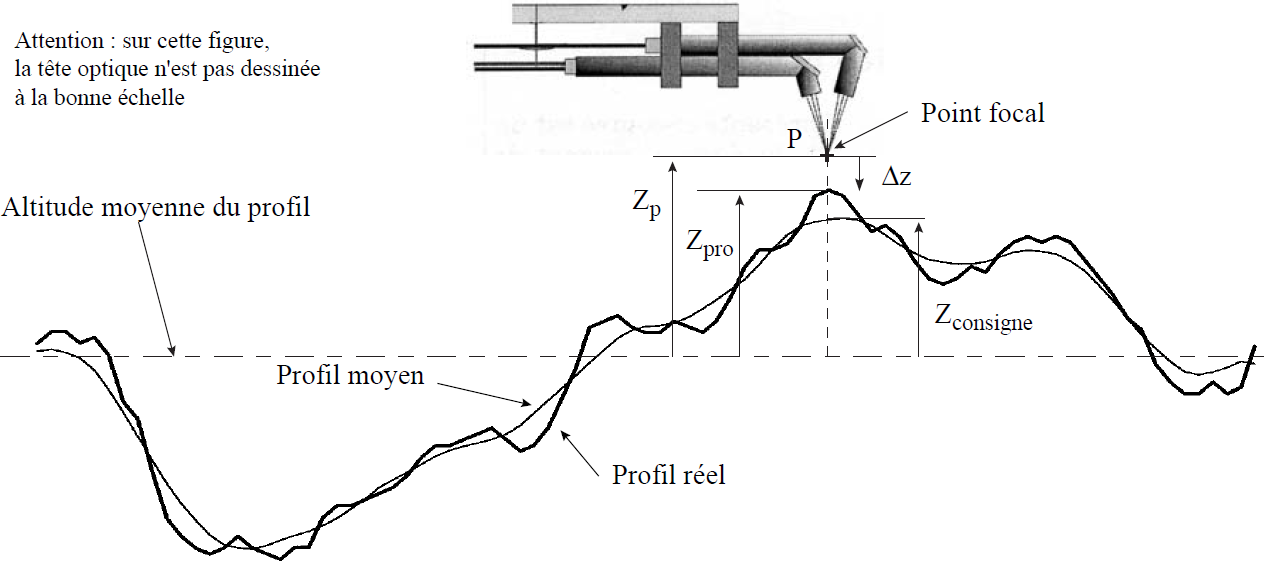
\includegraphics[width=\linewidth]{fig_08}
\caption{Asservissement en vitesse et position de l’axe A1\label{kuka:fig:08}}
\end{figure}

Les performances souhaitées sont les suivantes : 
\begin{itemize}
\item pas d’écart de position, écart de traînage lors d’un transfert à \SI{105}{\degres/s} inférieur à 1\degres ; 
\item marge de phase de 45\degres.
\end{itemize}
\fi

\subsection{Fonction de transfert du moteur}

\question{Donner l’expression littérale de l’inertie équivalente $J_e$ ramenée sur l’arbre 
moteur en fonction de $J_m$ et de $J_1$.}
\ifprof
\begin{corrige}
Non évaluée. On montrera plus tard que $J_e = J_m + \dfrac{J_1}{N^2}$...
\end{corrige}
\else
\fi

\question{Déterminer les transformées de Laplace des équations 1 à 4 du moteur 
définies au paragraphe \ref{sec:6:2} en considérant nulles les conditions initiales.}
\ifprof
\begin{corrige}
\begin{itemize}
\item $U(p) = RI(p) + E(p)$ (1);
\item $e(t) = k_e \Omega_m(p)$  (2);
\item $J_e p \Omega_m(p) = C_m(p)$ (3);
\item $C_m(p) = k_t I(p)$ (4).
\end{itemize}
\end{corrige}
\else
\fi

\question{Recopier et compléter le schéma bloc suivant avec les transmittances manquantes. }
\ifprof
\begin{corrige} ~\\

\begin{center}
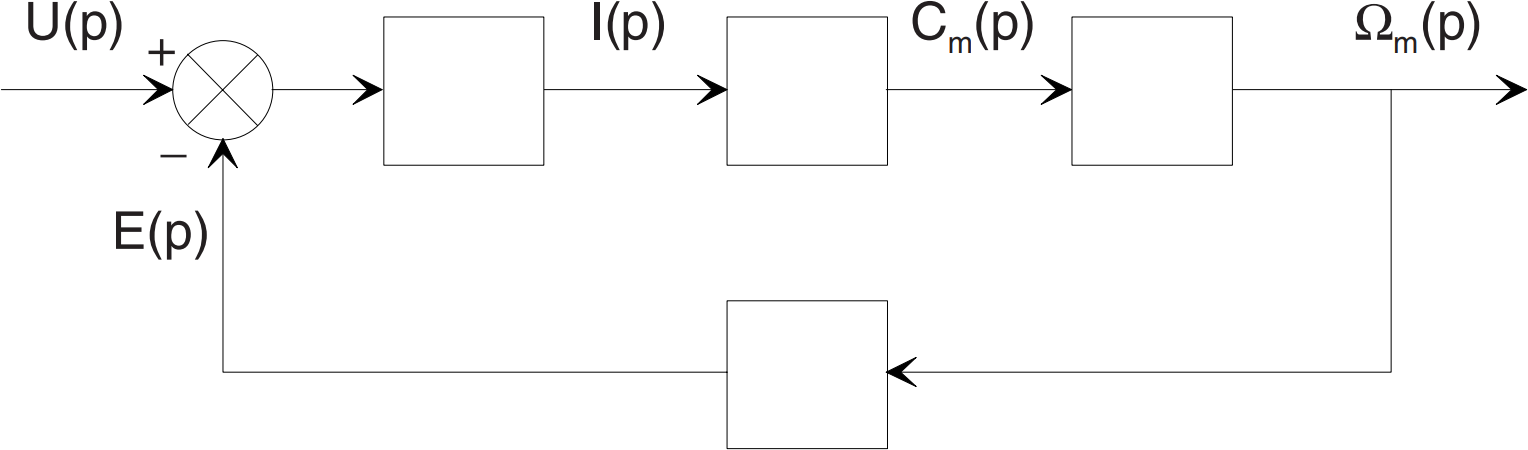
\includegraphics[width=.7\linewidth]{dr_03}
\end{center}\end{corrige}
\else

\begin{center}
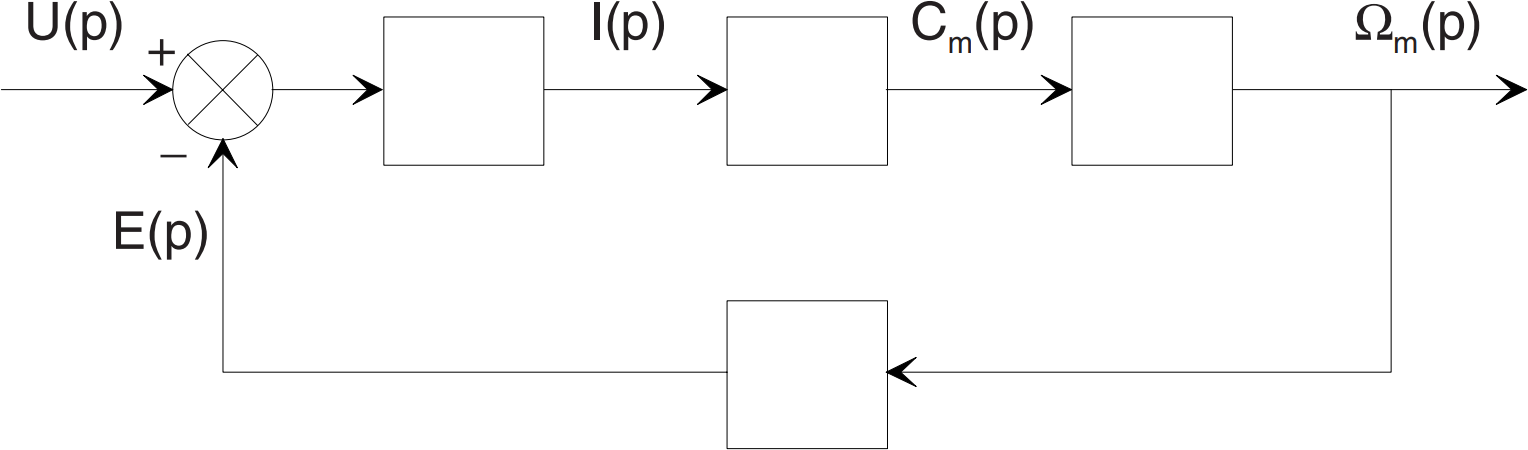
\includegraphics[width=.7\linewidth]{dr_03}
\end{center}
\fi





\question{En déduire la fonction de transfert $M(p)=\dfrac{\Omega(p)}{U(p)}$ du moteur que l’on 
exprimera sous la forme canonique d’un système du premier ordre de gain $K_m$ et de 
constante de temps $\tau_m$. Donner les expressions littérales de $K_m$ et $\tau_m$ et préciser leurs unités. }
\ifprof
\begin{corrige}
On a $M(p)=\dfrac{\dfrac{1}{k_e}}{\dfrac{RJ_e}{k_t k_e}p+1}$ 
avec $\tau_m = \dfrac{RJ_e}{k_t k_e}$ (\si{s})
et $k_m = \dfrac{1}{k_e}$ (\si{rad.s^{-1}V^{-1}}).
\end{corrige}
\else
\fi

\question{Calculer, suivant l’inertie $J_e$ mini ou maxi du robot, les caractéristiques 
suivantes du moteur.}
\vspace{-.4cm}
\textit{\begin{enumerate}
\item constante de temps $\tau_m$ (mini et maxi) ; 
\item temps de réponse à 5\% (mini et maxi) ; 
\item bande passante à \SI{-3}{dB} (mini et maxi) ; 
\end{enumerate}
Conclure quant à l’influence de l’inertie du robot sur les performances du moteur. }
\ifprof
\begin{corrige}
$\tau_m = \SI{0,3}{s}$ ou $\tau_m = \SI{0,45}{s}$. 

$t_5 = \SI{0,9}{s}$ ou $\tau_m = \SI{1,35}{s}$.

$\omega_c = \dfrac{1}{\tau_m} = \SI{3,08}{rad.s^{-1}}$ ou $\omega_c = \dfrac{1}{\tau_m} = \SI{2,22}{rad.s^{-1}}$. 

Plus l’inertie équivalente est importante, plus le système est lent.
\end{corrige}
\else
\fi


\subsection{Étude de la boucle de vitesse}
La tension $u_g(t)$ en sortie de la génératrice tachymétrique varie de 0 à \SI{12}{V} quand la vitesse de 
rotation du moteur varie de 0 à \SI{3500}{tr.min^{-1}}.
 
\question{En déduire la valeur du gain $K_g$ de la génératrice tachymétrique.}
\ifprof
\begin{corrige}
$k_g = \dfrac{12}{3600}\dfrac{60}{2\pi} = \SI{3,27e-3}{V.rad^{-1}.s}$.
\end{corrige}
\else
\fi

\question{Déterminer, en fonction notamment de $K_m$ et $\tau_m$, la fonction de transfert $H(p)=\dfrac{\Omega_m(p)}{U_v(p)}$ que l’on exprimera sous la forme canonique d’un système du premier ordre de gain $K_m'$ et de constante de temps $\tau_m'$. Donner les expressions littérales de $K_m'$ et $\tau_m'$ et préciser leurs unités.}
\ifprof
\begin{corrige}
$H(p)=\dfrac{G k_m}{1+\tau_m p + Gk_m k_g}$ et $k'_m = \dfrac{Gk_m}{2+Gk_mk_g}$ en $\si{V.rad^{-1}.s^{-1}}$
et $\tau'_m = \dfrac{\tau_m}{1+Gk_mk_g}$ en s.
\end{corrige}
\else
\fi

\question{Montrer que, si $G$ est très grand, on peut admettre que  $H(p)\simeq \dfrac{1}{K_g}$.}
\ifprof
\begin{corrige}
Calculer la limite lorsque G tend vers l'infini.
\end{corrige}
\else
\fi

\subsection{Étude de la boucle de position}
\ifprof
\else
La boucle de position est représentée Figure 9 ci-dessous. On admet que : 
\begin{itemize}
\item $H(p)=\dfrac{\Omega_m(p)}{U_v(p)} = \dfrac{30}{1+5\times 10^{-3}p}$;
\item $K_r = \SI{4}{V/rad}$ : gain du capteur de position;
\item $K_a$ : gain de l'adaptateur du signal de consigne $\alpha_e(t)$;
\item le signal de consigne $\alpha_e(t)$ est exprimé en degré;
\item le correcteur $C(p)$ est à action proportionnelle de gain réglable $K_c$.
\end{itemize}

\begin{figure}[!h]
\centering
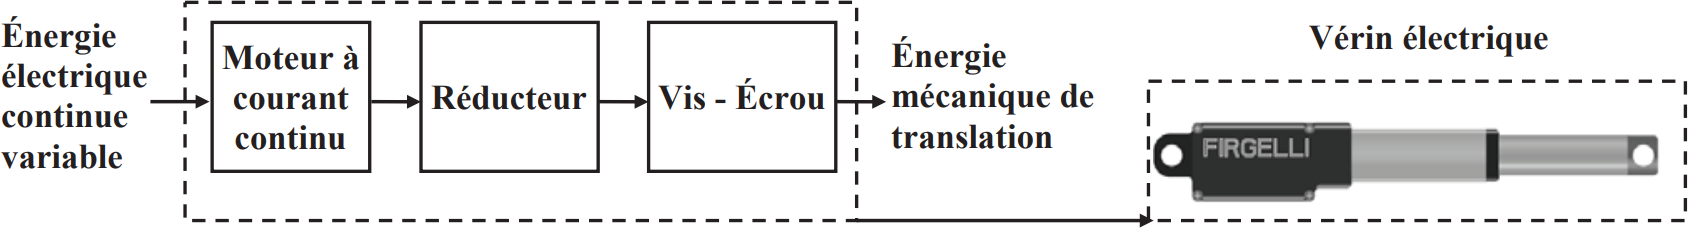
\includegraphics[width=.9\linewidth]{fig_09}
\caption{Boucle de position\label{kuka:fig:09}}
\end{figure}
\fi

\question{Déterminer la fonction de transfert $R(p)=\dfrac{\alpha_r(p)}{\Omega_m(p)}$ du réducteur.}
\ifprof
\begin{corrige}
$R(p) = \dfrac{1}{Np}$
\end{corrige}
\else
\fi

\question{Déterminer le gain $K_a$ de l'adaptateur.}
\ifprof
\begin{corrige}
$k_a = \dfrac{\pi}{180} k_r = \SI{6,98e-2}{V/\degres}$.
\end{corrige}
\else
\fi

\question{Déterminer, en fonction notamment de $K_m'$ et $\tau_m'$, la fonction de transfert 
en boucle ouverte $T(p)$ que l’on exprimera sous forme canonique. En déduire l’expression du 
gain de boucle, noté $\indice{K}{BO}$.}
\ifprof
\begin{corrige}
$T(p)=\dfrac{\dfrac{k_c k'_m k_r}{N}}{p(1+\tau'_m p)}$ et $\indice{k}{BO}=\dfrac{k_c k'_m k_r}{N}$.
\end{corrige}
\else
\fi

On souhaite une marge de phase de 45\degres.

\question{\label{q:6:11a} Déterminer la valeur de $\indice{K}{BO}$ permettant de satisfaire cette condition.}
\ifprof
\begin{corrige}
\end{corrige}
\else
\fi
\question{\label{q:6:11b} En déduire la valeur du gain $K_c$ du correcteur.}
\ifprof
\begin{corrige}
\end{corrige}
\else
\fi
\question{\label{q:6:11c} Déterminer l’écart de position. Conclure vis-à-vis des exigences du cahier des 
charges.}
\ifprof
\begin{corrige}
Classe 1 donc écart en position nul.
\end{corrige}
\else
\fi
On souhaite un écart de traînage inférieur à 1\degres pour une consigne de vitesse de \SI{105}{\degres/s}. 

\question{Déterminer l’expression de $\alpha_e(t)$ correspondant à une consigne de vitesse de \SI{105}{\degres/s}. En déduire $\alpha_e(p)$.}
\ifprof
\begin{corrige}
$\alpha_e(p) = \dfrac{105}{p^2}$.
\end{corrige}
\else
\fi

\question{La valeur de $\indice{K}{BO}$ définie question \ref{q:6:11a} permet-elle de satisfaire l’exigence 
de précision imposée par le cahier des charges ? Conclure.}
\ifprof
\begin{corrige}
$\varepsilon_d = 105 k_a/\indice{K}{BO} = \SI{0,025}{V}$.
\end{corrige}
\else
\fi


